\documentclass[preview]{standalone}

\usepackage{amsmath}
\usepackage{amssymb}
\usepackage{tikz}
\usepackage{pgfplots}
\usepackage{wrapfig}
\usepackage{stellar}
\usepackage{definitions}
\usepackage{bettelini}
\usepackage{xfrac}

\usetikzlibrary{positioning, arrows.meta}

\begin{document}

\id{definite-integrals}
\genpage

\section{Step functions}

\begin{snippetdefinition}{indicator-function-definition}{Indicator function}
    Let \(A\) be a \set.
    The \textit{indicator function} of \(A\) is defined as
    \[
        1_{A}(x) \triangleq \begin{cases}
            1 & x \in A \\
            0 & x \notin A
        \end{cases}
    \]
\end{snippetdefinition}

\begin{snippetdefinition}{function-positive-part-definition}{Function positive part}
    Let \(f(x)\) be a real-valued \function.
    The \emph{positive part} of \(f(x)\) is defined as
    \[
        f^+(x) = \max\{f(x), 0\}
    \]
\end{snippetdefinition}

\begin{snippetdefinition}{function-negative-part-definition}{Function negative part}
    Let \(f(x)\) be a real-valued \function.
    The \emph{negative part} of \(f(x)\) is defined as
    \[
        f^-(x) = -\min\{f(x), 0\}
    \]
\end{snippetdefinition}

\begin{snippetproposition}{positive-negative-part-property}{}
    Let \(f(x)\) be a real-valued \function. Then,
    \[
        f^+ = \frac{|f| + f}{2}, \qquad
        f^- = \frac{|f| - f}{2}
    \]
\end{snippetproposition}

\begin{snippetdefinition}{step-function-definition}{Step function}
    Let \(f\colon \realnumbers \fromto \realnumbers\) be a \function. Then, \(f\) is a \emph{step function}
    if it can be written as
    \[
        f(x) = \sum_{i=0}^n \alpha_i \indicator_{A_i}(x)
    \]
    where \(\alpha_i\in\realnumbers\) and \(A_i\) is a partition of intervals.
    Such a partition is called an \emph{adapted partition} of \(f\).
    If the partition assumes different values in consecutive intervals, the partition is called
    an \emph{induced partition} of \(f\).
\end{snippetdefinition}

\plain{The induced partition is the minimal partition that can be used to represent a step function.}

\begin{snippetproposition}{step-functions-properties}{Step function properties}
    Let \(\varphi, \psi\colon I \fromto \realnumbers\) be \stepfunction[step functions].
    Then,
    \begin{enumerate}
        \item there exist a partition that is an adapted partition of both \(\varphi\) and \(\psi\),
        \item \(\alpha\varphi + \beta\psi\) is a \stepfunction for any \(\alpha, \beta \in \realnumbers\),
        \item given a family of subintervals \(\{J_l\}\) of \(I\) and \(\gamma_l \in \realnumbers\),
        \[
            \sum_{l=1}^n \gamma_l \indicator_{J_l}
        \]
        is a \stepfunction.
        \item \(\varphi\psi\) and \(\varphi/\psi\) if \(\psi(x) \neq 0\) are \stepfunction[step functions].
        \item let \(F\colon A \subseteq \realnumbers \fromto \realnumbers\) be a \function
        such that \(\varphi(I) \subseteq A\), then \(F\circ\varphi\) is a \stepfunction.
        In particular, \(\varphi^+\) and \(\varphi^-\) are \stepfunction[step functions].
    \end{enumerate}
\end{snippetproposition}

\begin{snippetdefinition}{integral-of-step-function-definition}{Integral of step function}
    Let \(\varphi\colon \Omega \fromto \realnumbers\) be a \stepfunction[step function]
    and \(\{I_k\}\) be an adapted partition of \(\varphi\) such that
    \[
        \varphi = \sum_{k=1}^n \alpha_k \indicator_{I_k}
    \]
    Then,
    \[
        \int_\Omega \varphi = \sum_{k=1}^n \alpha_k \mu(I_k)
    \]
    where \(\mu\) is the length of the interval.
\end{snippetdefinition}

\begin{snippet}{integral-of-step-function-induced-partition}
    It is not necessary to choose a partition induced by \(\varphi\) but any adapted partition
    suffices. The adapted partition is created by dividing the intervals in the induced partition.
    Let \(\{I_k\}\) be an adapted partition of \(\varphi\) and \(\{J_i\}\) be an induced partition of \(\varphi\)
    such that
    \[
        I_k = \bigcup_{i=1}^{n_k} J_{k_i}
    \]
    and \(\varphi(x) = \alpha_k\) on \(I_k\) where \(J_i\) are disjoint intervals.
    Then,
    \[
        \alpha_k \cdot \mu(I_k) = \sum_{i=1}^{n_k} \alpha_k \mu(J_{k_i})
    \]
    and \(\{J_{k_i}\}\) is an adapted partition of \(\varphi\) and
    \[
        \varphi(x) = \sum_{i=1} \alpha_i 1_{J_{k_i}}
    \]
    which means that
    \[
        \sum_{i=1} \alpha_i \mu(J_{k_i}) = \sum_{k=1} \alpha_k \mu(I_k)
    \]
    and the integral remains the same.
\end{snippet}

\begin{snippetproposition}{step-function-integral-properties}{Step function integral properties}
    Let \(\varphi, \psi\colon \Omega \fromto \realnumbers\) be \stepfunction[step functions].
    Then,
    \begin{enumerate}
        \item \emph{linearity:}
            \[
                \int_\Omega \left( \alpha\varphi + \beta\psi \right) = \alpha\int_\Omega \varphi + \beta\int_\Omega \psi
            \]
            for any \(\alpha, \beta \in \realnumbers\).
        \item \emph{monotonicity:}
            \[
                \varphi \leq \psi \implies \int_\Omega \varphi \leq \int_\Omega \psi
            \]
        \item \emph{triangular inequality:}
            \[
                \left| \int_\Omega \varphi \right| \leq \int_\Omega |\varphi|
            \]
        \item let \(\Omega = \Omega_1 \union \Omega_2\) where \(\Omega_1 \intersection \Omega_2 = \emptyset\). Then,
            \[
                \int_\Omega \varphi = \int_{\Omega_1} \varphi + \int_{\Omega_2} \varphi
            \]
        \item if \(\varphi(x) = \psi(x)\) except in a finite number of points, then
            \[
                \int_\Omega \varphi = \int_\Omega \psi
            \]
    \end{enumerate}
\end{snippetproposition}

\begin{snippetproof}{step-function-integral-properties-proof}{step-function-integral-properties}{Step function integral properties}
    \begin{enumerate}
        \item \emph{linearity:} let \(\{J_i\}\) be a partition adapted to both \(\varphi\) and \(\psi\)
        such that
        \[
            \varphi = \sum_{i=1}^n \alpha_i \indicator_{J_i}, \qquad
            \psi = \sum_{i=1}^n \beta_i \indicator_{J_i}
        \]
        Then,
        \[
            \alpha\varphi + \beta\psi = \sum_{i=1}^n (\alpha\alpha_i + \beta\beta_i) \indicator_{J_i}
        \]
        and the integrals are given by splitting the sum and applying the integral of a \stepfunction.
        \item \emph{monotonicity:} let \(\{J_i\}\) be a partition adapted to both \(\varphi\) and \(\psi\)
        such that
        \[
            \varphi = \sum_{i=1}^n \alpha_i \indicator_{J_i}, \qquad
            \psi = \sum_{i=1}^n \beta_i \indicator_{J_i}
        \]
        We have that \(\varphi(x) \leq \psi(x)\) for \(x\in\Omega\) \ifandonlyif \(\alpha_k \leq \beta_k\) for all \(k\).
        Thus, the integral of \(\varphi\) is less than the integral of \(\psi\)
        \[
            \int_\Omega \varphi = \sum_{i=1}^n \alpha_i \mu(J_i) \leq \sum_{i=1}^n \beta_i \mu(J_i) = \int_\Omega \psi
        \]
        In particular, if \(\psi \geq 0\) on \(\Omega\) then
        \[
            \int_\Omega \psi \geq 0
        \]
        \item 
    \end{enumerate}
\end{snippetproof}

\begin{snippetdefinition}{dirichlet-function-definition}{Dirichlet function}
    The \emph{Dirichlet function} is defined as \(\indicator_{\rationalnumbers}\).
\end{snippetdefinition}

\section{Riemann integral}

\begin{snippetdefinition}{riemann-integral-definition}{Riemann integral}
    Let \(\varphi\colon \Omega \fromto \realnumbers\) be a \bounded \function
    on a \bounded interval \(\Omega\).
    The \emph{lower Riemann integral} is defined as
    \[
        \lrint_\Omega \varphi = \sup\left\{ \int_\Omega \psi \suchthat \psi \leq \varphi \text{ on } \Omega \land \varphi \in \setofstepfunctions \right\}
    \]
    The \emph{upper Riemann integral} is defined as
    \[
        \urint_\Omega \varphi = \inf\left\{ \int_\Omega \psi \suchthat \psi \geq \varphi \text{ on } \Omega \land \varphi \in \setofstepfunctions \right\}
    \]
    Then, \(\varphi\) is \emph{Riemann integrable} on \(\Omega\) if
    \[
        \urint_\Omega \varphi = \lrint_\Omega \varphi
    \]
    and we define
    \[
        R-\hspace{-0.1cm}\int_\Omega \varphi \triangleq \lrint_\Omega \varphi = \urint_\Omega \varphi
    \]
    \emph{Syntax:} let \(\Omega = (a,b)\) where the endpoints can also be included in the interval
    \[
        \int\limits_a^b f \triangleq \begin{cases}
            \int_\Omega f & a<b \\
            0 & a=b \\
            - \int_\Omega f & b<a
        \end{cases}
    \]
\end{snippetdefinition}

\begin{snippetlemma}{step-functions-are-riemann-integrable}{}
    Let \(f\colon \Omega \fromto \realnumbers\) be a \stepfunction[step function].
    Then, \(f\) is Riemann integrable on \(\Omega\) and
    \[
        R-\hspace{-0.1cm}\int_\Omega f = \int_\Omega f
    \]
\end{snippetlemma}

\begin{snippetproof}{step-functions-are-riemann-integrable-proof}{step-functions-are-riemann-integrable}{}
    We need to show that if \(f\) is a \stepfunction then
    \[
        \int_\Omega f
        = \sup\left\{ \int_\Omega \psi \suchthat \psi \leq f \text{ on } \Omega \land f \in \setofstepfunctions \right\}
        = \inf\left\{ \int_\Omega \psi \suchthat \psi \geq f \text{ on } \Omega \land f \in \setofstepfunctions \right\}
    \]
    Without loss of generality, we will verify the first equality.
    For every \stepfunction \(\psi\) such that \(\psi \leq f\), we have that
    \[
        \int_\Omega \psi \leq \int_\Omega f
    \]
    and by using the supremum on \(\psi\) we have
    \[
        \sup\left\{ \int_\Omega \psi \suchthat \psi \leq f \text{ on } \Omega \land f \in \setofstepfunctions \right\}
        \leq \int_\Omega f
    \]
    On the other hand, since \(f\) is a \stepfunction, \(f\) is one of the \stepfunction[step functions]
    that we are considering, meaning
    \[
        \int_\Omega f \leq
        \sup\left\{ \int_\Omega \psi \suchthat \psi \leq f \text{ on } \Omega \land f \in \setofstepfunctions \right\}
        \leq \int_\Omega f
    \]
    which gives the equality.
\end{snippetproof}

\begin{snippettheorem}{dirichlet-function-not-riemann-integrable-theorem}{}
    The Dirichlet function \(1_{\rationalnumbers}\) is not Riemann integrable on \([a,b]\).
\end{snippettheorem}

\begin{snippetproof}{dirichlet-function-not-riemann-integrable-theorem-proof}{dirichlet-function-not-riemann-integrable-theorem}{}
    We will separately compute the upper and lower Riemann integrals.
    \begin{itemize}
        \item we know that \(1_{\rationalnumbers} \geq 0\) and by definition of lower Riemann integral
        \[
            \lrint_{[a,b]} 1_{\rationalnumbers} = \sup\left\{ \int_{[a,b]} \varphi \suchthat \varphi \leq 1_{\rationalnumbers} \land \varphi \in \setofstepfunctions \right\}
            \leq \int_\Omega 1_{\rationalnumbers} \geq \int_\Omega 0 = 0
        \]
        On the other hand, let
        \[
            \varphi = \sum_{k=1}^n \alpha_k \indicator_{\Omega_k}
        \]
        be a \stepfunction such that \(\varphi \leq 1_{\rationalnumbers}\) on \([a,b]\)
        where \(\{\Omega_k\}\) is a partition of \(\Omega = [a,b]\), meaning
        \[
            \bigcup_k \Omega_k = \Omega = [a,b]
        \]
        where \(\Omega_i\) are \disjoint. By definition we have
        \begin{align*}
            \int_\Omega \varphi &=
            \sum_{k=1}^n \alpha_k \mu(\Omega_k) \\
            &= \sum_{\substack{k=1 \\ \mu(\Omega_k) > 0}}^n \alpha_k \mu(\Omega_k)
            + \sum_{\substack{k=1 \\ \mu(\Omega_k) = 0}}^n \alpha_k \mu(\Omega_k) \\
            &= \sum_{\substack{k=1 \\ \mu(\Omega_k) > 0}}^n \alpha_k \mu(\Omega_k)
        \end{align*}
        Since \(\realnumbers\) and \(\realnumbers \difference \rationalnumbers\) are dense in \(\mathbb{R}\),
        every interval \(\Omega_k\) such that \(\mu(\Omega_k) > 0\) contains infinite rational and irrational numbers.
        In particular, there exist \(x_k\in \Omega_k\) such that \(x_k \in \realnumbers \difference \rationalnumbers\)
        and since \(\varphi\leq 1_{\rationalnumbers}\) we have that
        \[
            \varphi(x_n) \leq 1_{\rationalnumbers}(x_n) = 0
        \]
        Thus, for every \(k\), \(\mu(\Omega_k) \geq 0\) and \(\alpha_k \leq 0\) and by substituting in the integral
        we have
        \[
            \int_\Omega \varphi \leq 0
        \]
        for every \stepfunction \(\varphi\) such that \(\varphi \leq 1_{\rationalnumbers}\) on \([a,b]\).
        We then use the supremum
        \[
            \lrint_{[a,b]} 1_{\rationalnumbers} \leq 0 \implies \lrint_{[a,b]} 1_{\rationalnumbers} = 0
        \]
        \item we know that \(1_{\rationalnumbers} \leq 1\) and by definition of upper Riemann integral
        \[
            \urint_{[a,b]} 1_{\rationalnumbers} = \inf\left\{ \int_{[a,b]} \psi \suchthat \psi \geq 1_{\rationalnumbers} \land \psi \in \setofstepfunctions \right\}
            \leq \int_\Omega 1_{\rationalnumbers} = \mu(\Omega)
        \]
        On the other hand, let
        \[
            \psi = \sum_{k=1}^n \beta_k \indicator_{\Omega_k}
        \]
        be a \stepfunction like before. Then,
        \[
            \int_\Omega \psi = \sum_{k=1}^n \beta_k \mu(\Omega_k) =
            \sum_{\substack{k=1 \\ \mu(\Omega_k) > 0}}^n \beta_k \mu(\Omega_k)
        \]
        meaning that for each \(k\) we have \(\mu(\Omega_k) > 0\) there exist
        \(x_k'\in \Omega_k\) such that \(x_k' \in \rationalnumbers\) from which
        \[
            \beta_k = \psi(x_k') \geq 1_{\rationalnumbers}(x_k') = 1
        \]
        and by substituting in the definition we have
        \begin{align*}
            \int_\Omega \psi &= \sum_{\substack{k=1 \\ \mu(\Omega_k) > 0}}^n \beta_k \mu(\Omega_k) \\
            &\geq \sum_{\substack{k=1 \\ \mu(\Omega_k) > 0}}^n \beta_k \mu(\Omega_k) 
            = \sum_{k=1}^n \beta_k \mu(\Omega_k) = \mu(\Omega_k)
        \end{align*}
        which means that \(\forall \psi \geq 1_{\rationalnumbers}\) \stepfunction[step function] on \([a,b]\)
        \[
            \int_\Omega \psi \geq \mu(\Omega)
        \]
        and by using the infimum we have
        \[
            \urint_{[a,b]} 1_{\rationalnumbers}
            = \inf\left\{ \int_{[a,b]} \psi \suchthat \psi \geq 1_{\rationalnumbers} \land \psi \in \setofstepfunctions \right\}
            \geq \mu(\Omega) = \mu(\Omega)
        \]
    \end{itemize}
    Thus, such a \function is not Riemann integrable on \([a,b]\).
\end{snippetproof}

\begin{snippettheorem}{riemann-integrability-equivalence-theorem}{Riemann integrability equivalences}
    Let \(f\colon \Omega \fromto \realnumbers\) bounded on \(\Omega\) bounded interval.
    The following are equivalent:
    \begin{enumerate}
        \item \(f\) is Riemann integrable on \(\Omega\);
        \item \(\forall \varepsilon > 0, \exists \varphi_\varepsilon, \psi_\varepsilon\)
        \stepfunction[step functions] such that \(\varphi_\varepsilon \leq f \leq \psi_\varepsilon\) and
        \[
            0 \leq
            \int_\Omega (\psi_\varepsilon - \varphi_\varepsilon)
            < \epsilon
        \]
        \item There exist \sequence[sequences] of \stepfunction[step functions] \(\{\varphi_n\}\)
        and \(\{\psi_n\}\) such that for every \(n\), \(\varphi_n \leq f \leq \psi_n\) on \(\Omega\)
        and
        \[
            0 \leq \int_\Omega (\psi_n - \varphi_n) \to 0
        \]
        for \(n\to \infty\).
        Furthermore, there exist
        \[
            \lim_n \int_\Omega \varphi_n = \lim_n
            \int_\Omega \psi_n = \int_\Omega f
        \]
    \end{enumerate}
\end{snippettheorem}

\begin{snippetproof}{riemann-integrability-equivalence-theorem-proof}{riemann-integrability-equivalence-theorem}{Riemann integrability equivalences}
    \begin{enumerate}
        \item \((1) \implies (2)\): let \(f\) be Riemann integrable.
        By definition,
        \begin{align*}
            \lrint_\Omega f &= \sup\left\{
                \int_\Omega \varphi \mid \varphi \in \setofstepfunctions \land \varphi \leq f \text{ on } \Omega
            \right\} \\
            &= \inf\left\{
                \int_\Omega \varphi \mid \varphi \in \setofstepfunctions \land \varphi \geq f \text{ on } \Omega
            \right\} \\
            &= \urint_\Omega f = \int_\Omega f
        \end{align*}
        By defintion of (finite) infimum and supremum \(\forall \varepsilon>0\)
        there exist \(\varphi_\varepsilon\) \stepfunction with \(\varphi_\varepsilon \leq f\) on \(\Omega\)
        such that
        \[
            \int_\Omega \varphi_\varepsilon > \lrint_\Omega f - \frac{\varepsilon}{2} = \int_\Omega f - \frac{\varepsilon}{2}
        \]
        and likewise there exist \(\psi_\varepsilon\) \stepfunction with \(\psi_\varepsilon \geq f\) on \(\Omega\)
        such that
        \[
            \int_\Omega \psi_\varepsilon < \urint_\Omega f + \frac{\varepsilon}{2} = \int_\Omega f + \frac{\varepsilon}{2}
        \]
        From this it follows
        \[
            0 \leq \int_\Omega \psi_\varepsilon - \int_\Omega \varphi_\varepsilon <
            \left(
                \int_\Omega f + \frac{\varepsilon}{2}
            \right) -
            \left(
                \int_\Omega f - \frac{\varepsilon}{2}
            \right)
            = \frac{\varepsilon}{2} + \frac{\varepsilon}{2} = \varepsilon
        \]
        \item \((2) \implies (3)\): by hypothesis \(\forall \varepsilon > 0, \exists \varphi_\varepsilon, \psi_\varepsilon\)
        \stepfunction[step functions] such that \(\varphi_\varepsilon \leq f \leq \psi_\varepsilon\) on \(\Omega\) and
        \[
            0 \leq \int_\Omega \psi_\varepsilon - \int_\Omega \varphi_\varepsilon < \varepsilon
        \]
        Let \(\varepsilon = \frac{1}{n}\), for every \(n\) there exist
        \(\varphi_\varepsilon, \psi_\varepsilon\) \stepfunction[step functions] where \(\varphi_n \leq f \leq \psi_n\)
        on \(\Omega\) and
        \[
            0 \leq \int_\Omega \psi_n - \int_\Omega \varphi_n < \frac{1}{n} \to 0
        \]
        \item \((3) \implies (1)\): By hypothesis there exist
        \(\{\varphi_n\}\) and \(\{\psi_n\}\) \sequence of \stepfunction[step functions] such that for every \(n\),
        \(\varphi_n \leq f \leq \psi_n\) and
        \[
            0 \leq \int_\Omega \psi_n - \int_\Omega \varphi_n \to 0
        \]
        By definition, for every \(n\) we have
        \[
            \lrint_\Omega f = \sup\left\{
                \int_\Omega \varphi \mid \varphi \in \setofstepfunctions \land \varphi \leq f \text{ on } \Omega
            \right\} \geq \int_\Omega \varphi_n
        \]
        and
        \[
            \urint_\Omega f = \inf\left\{
                \int_\Omega \varphi \mid \varphi \in \setofstepfunctions \land \varphi \geq f \text{ on } \Omega
            \right\} \leq \int_\Omega \psi_n
        \]
        from which
        \[
            0 \leq \urint_\Omega f - \lrint_\Omega f \leq
            \int_\Omega \psi_n - \int_\Omega \varphi \to 0
        \]
        meaning that \(\urint_\Omega f\) must be equal to \(\lrint_\Omega f\) and thus \(f\)
        is Riemann integrable. Furthermore, we have that
        \[
            0 \leq \lrint_\Omega f - \int_\Omega \varphi_n = \int_\Omega f - \int_\Omega \varphi_n
            \leq \int_\Omega \psi_n - \int_\Omega \varphi_n \to 0
        \]
        which proves that the following exists
        \[
            \lim_{n} \int_\Omega \varphi_n = \int_\Omega f
        \]
        and likewise for \(\psi_n\).
    \end{enumerate}
\end{snippetproof}

\begin{snippetproposition}{riemann-integral-properties}{Riemann integral properties}
    Let \(f,g\colon \Omega \fromto \realnumbers\) \bounded on a \bounded interval \(\Omega\). Then,
    \begin{enumerate}
        \item if \(f\) and \(g\) are Riemann integrable, then
        \begin{enumerate}
            \item \emph{linearity} \(\forall \alpha,\beta\), \(\alpha f+\beta g\) is Riemann integrable and
            \[
                \int_\Omega \alpha f+\beta g = \alpha\int_\Omega f + \beta\int_\Omega g
            \]
            \item \(fg\) is Riemann integrable and if \(1/g\) is bounded on \(\Omega\),
            \(f/g\) is also Riemann integrable on \(\Omega\).
        \end{enumerate}
        \item if \(f,g\) are Riemann integrable on \(\Omega\) and \(f \leq g\) on \(\Omega\), then
        \[
            \int_\Omega f \leq \int_\Omega g
        \]
        In particular, if \(g \geq 0\) on \(\Omega\),
        \[
            \int_\Omega g \geq 0
        \]
        \item \emph{triangular inequality} if \(f\) is Riemann integrable on \(\Omega\)
        then \(f^+\), \(f^-\) and \(|f|\) are Riemann integrable and
        \[
            \left|\int_\Omega f\right| \leq \int_\Omega |f|
        \]
        \item \emph{additivity with respect to the domain of integration}
        If \(\Omega = \Omega_1 \cup \Omega_2\) \disjoint, then \(f\) is Riemann integrable on \(\Omega\)
        \ifandonlyif it is Riemann integrable on \(\Omega_1\) and \(\Omega_2\), in which case
        \[
            \int_\Omega f = \int_{\Omega_1} f + \int_{\Omega_2} f
        \]
        In the case where \(\Omega = \Omega_1 \cup \Omega_2\) but the intervals are not necessarily
        \disjoint, then the riemann Integrability equivalence is still valid but
        \[
            \int_\Omega f = \int_{\Omega_1} f + \int_{\Omega_2} f - \int_{\Omega_1 \cap \Omega_2} f
        \]
        \item If \(f=g\) except in a finite amount of points, then \(f\)
        it is Riemann integrable \ifandonlyif \(g\) if Riemann integrable, in which case
        \[
            \int_\Omega f = \int_\Omega g
        \]
    \end{enumerate}
\end{snippetproposition}

\begin{snippetproof}{riemann-integral-properties-proof}{riemann-integral-properties}{Riemann integral properties}
    \begin{itemize}
        \item We prove that the addition is still Riemann integrable. For every \(\varepsilon>0\)
        there exist \stepfunction[step functions] \(\varphi_\varepsilon^f \leq f \leq \psi_\varepsilon^f\) on \(\Omega\)
        such that
        \[
            0 \leq \int_\Omega \psi_\varepsilon^f - \int_\Omega \varphi_\varepsilon^f < \frac{\varepsilon}{2}
        \]
        and \(\varphi_\varepsilon^g \leq g \leq \psi_\varepsilon^g\) on \(\Omega\) such that
        \[
            0 \leq \int_\Omega \psi_\varepsilon^g - \int_\Omega \varphi_\varepsilon^g < \frac{\varepsilon}{2}
        \]
        Consider their sum \(\varphi_\varepsilon = \varphi_\varepsilon^f + \varphi_\varepsilon^g\) and \(\psi_\varepsilon = \psi_\varepsilon^f + \psi_\varepsilon^g\)
        it follows that \(\varphi_\varepsilon\) and \(\psi_\varepsilon\) are \stepfunction[step functions] and
        \[
            \varphi_\varepsilon = \varphi_\varepsilon^f + \varphi_\varepsilon^g \leq f+g\leq \psi_\varepsilon^f + \psi_\varepsilon^g = \psi_\varepsilon
        \]
        and
        \begin{align*}
            0 \leq \int_\Omega \psi_\varepsilon - \int_\Omega \varphi_\varepsilon &< \int_\Omega \psi_\varepsilon^f + \int_\Omega \psi_\varepsilon^g - \int_\Omega \varphi_\varepsilon^f - \int_\Omega \varphi_\varepsilon^g \\
            &< \frac{\varepsilon}{2} + \frac{\varepsilon}{2} = \varepsilon
        \end{align*}
        and thus \(f+g\) is Riemann integrable. Furthermore, for every \(\varepsilon >0\)
        \[
            \int_\Omega (\varphi_\varepsilon^f + \varphi_\varepsilon^g) \leq \int_\Omega f+g \leq \int_\Omega (\psi_\varepsilon^f + \psi_\varepsilon^g)
        \]
        \[
            \int_\Omega \varphi_\varepsilon^f +\int_\Omega \varphi_\varepsilon^g \leq \int_\Omega f + \int_\Omega g \leq \int_\Omega \psi_\varepsilon^f + \int_\Omega\psi_\varepsilon^g
        \]
        da cui deduciamo che
        \begin{align*}
            \int_\Omega (f + g) - \left(
                \int_\Omega f + \int_\Omega g
            \right)
            \leq \int_\Omega \psi_\varepsilon^f + \int_\Omega \psi_\varepsilon^g
            - \left(
                \int_\Omega \varphi_\varepsilon^f + \int_\Omega \varphi_\varepsilon^g
            \right) = \varepsilon
        \end{align*}
        da cui concludiamo che
        \[
            \left|\int_\Omega (f+g) - \left(\int_\Omega f + \int_\Omega g\right)\right| < \varepsilon
        \]
        for every \(\varepsilon>0\).
        \item We now show that \(f^+\) is Riemann integrable.
        For every \(\varepsilon>0\) there exist \(\varphi_\varepsilon,\psi_\varepsilon\)
        \stepfunction[step functions] such that \(\varphi_\varepsilon \leq f \leq \psi_\varepsilon\) and
        \[
            0 \leq \int_\Omega \psi_\varepsilon - \int_\Omega \varphi_\varepsilon < \varepsilon
        \]
        Clearly, \(\varphi_\varepsilon^+ \leq f^+ \leq \psi_\varepsilon^+\)
        and thus
        \[
            0\leq \int_\Omega \psi_\varepsilon^+ - \int_\Omega \varphi_\varepsilon^+ \leq \int_\Omega \psi_\varepsilon - \int_\Omega \varphi_\varepsilon < \varepsilon
        \]
        Which means that it is Riemann integrable.
        Likewise, we can show that \(f^-\) is Riemann integrable.
        \item Since \(|f| = f^+ - f^-\)
        \[
            \left|\int_\Omega f\right|
            = \left|\int_\Omega (f^+ - f^-)\right|
            = \left|\int_\Omega f^+ - \int_\Omega f^-\right|
        \]
        and by the triangular inequality it is less than or equal to
        \begin{align*}
            \leq \left|\int_\Omega f^+\right|
            + \left|\int_\Omega f^-\right|
            = \int_\Omega f^+ + \int_\Omega f^- = \int (f^+ + f^-)
            = \int_\Omega |f|
        \end{align*}
    \end{itemize}
\end{snippetproof}

% lista di funzioni integrali


\subsection{Fundamental Theorem of Calculus}

\begin{snippettheorem}{fundamental-theorem-of-calculus}{Fundamental Theorem of Calculus}
    Let \(f\colon [a,b] \fromto \realnumbers\) be integrable on \([a,b]\)
    and let
    \[
        F(x) = \integral[a][x][f(t)][t]
    \]
    be its integral function centered in \(a\).
    Then:
    \begin{enumerate}
        \item \(F\) is Lipschitz continuous on \([a,b]\);
        \item if \(f\) is continuous on \(x_0 \in [a,b]\) then \(F\)
        is differentiable in \(x_0\) and
        \[
            F'(x_0) = f(x_0)
        \]
        \item if \(f\) is continuous on \([a,b]\) then \(F\) is a \primitivefunc of \(f\) on \([a,b]\);
        \item if \(f\) is continuous on \([a,b]\) and \(G\) is a \primitivefunc of \(f\)
        %(che per il punto precedente esiste, quindi qua stiamo dimostrando che se è continua esiste la primitiva)
        then \(\forall x \in [a,b]\)
        \[
            F(x) = \int\limits_a^x f(t)\,dt = G(x) - G(a)
        \]
        and in particular
        \[
            F(b) = \int\limits_a^b f(t)\,dt = G(b) - G(a)
        \]
    \end{enumerate}
\end{snippettheorem}

\begin{snippetproof}{fundamental-theorem-of-calculus-proof}{fundamental-theorem-of-calculus}{Fundamental Theorem of Calculus}
    \begin{enumerate}
        \item by hypothesis \(f\) is integrable on \([a,b]\) and in particular it is \bounded,
        meaning \(\exists M\) such that \(|f(t)| \leq M\) for every \(t\in [a,b]\).
        Given \(x,x' \in [a,b]\), assume without loss of generality \(x<x'\), we have
        \begin{align*}
            |F(x') - F(x)| &= \left|
                \int\limits_a^{x'} f(t)\,dt -
                \int\limits_a^x f(t)\,dt
            \right| \\
            &= \left|
                \int\limits_a^x f(t)\,dt +
                \int\limits_x^{x'} f(t)\,dt -
                \int\limits_a^x f(t)\,dt
            \right| \\
            &= \left|
                \int\limits_x^{x'} f(t)\,dt
            \right|
            = \left|\,
                \int\limits_{[x,x']} f(t)\,dt
            \right| 
            \leq \int\limits_{[x,x']} |f(t)|\,dt \\
            &\leq M \cdot \int\limits_{[x,x']} 1\,dt = M(x'-x) = M|x'-x|
        \end{align*}
        \item Let \(f\) be continuous on \(x_0 \in [a,b]\). We show that \(F\) is differentiable in \(x_0\)
        with \(F'(x_0) = f(x_0)\) meaning that
        \[
            \frac{F(x_0 + h) - F(x_0)}{h} \to f(x_0)
        \]
        for \(h\to 0\). This can also be stated as
        \[
            \left|
                \frac{F(x_0 + h) - F(x_0)}{h} - f(x_0)
            \right| \to 0
        \]
        for \(h \to 0\).
        We can write \(\forall h \neq 0\)
        \begin{align*}
            \left|
                \frac{F(x_0 + h) - F(x_0)}{h} - f(x_0)
            \right| &= \left|
                \frac{1}{h} \cdot \left(
                    \int\limits_a^{x_0 + h} f(t) \,dt -
                    \int\limits_a^{x_0} f(t) \,dt
                \right) - f(x_0)
            \right| \\
            &= \left|
                \frac{1}{h} \cdot \left(
                    \int\limits_{x_0}^{x_0 + h} f(t) \,dt -
                    hf(x_0)
                \right)
            \right| \\
            &= \left|
                \frac{1}{h} \cdot \left(
                    \int\limits_{x_0}^{x_0 + h} f(t) \,dt -
                    \int\limits_{x_0}^{x_0 + h} f(x_0)\,dt
                \right)
            \right| \\
            &= \left|
                \frac{1}{h}
                \int\limits_{x_0}^{x_0 + h} f(t) - f(x_0) \,dt
            \right|
        \end{align*}
        If \(h>0\), % (la disuglianza triangolare vale quando l'estremo superiore è maggiore a quello inferiore),
        then
        \begin{align*}
            \left|
                \frac{1}{h}
                \int\limits_{x_0}^{x_0 + h} f(t) - f(x_0) \,dt
            \right| &\leq \frac{1}{h} \int\limits_{x_0}^{x_0 + h} |f(t) - f(x_0)| \,dt
        \end{align*}
        By hypothesis, \(f\) is continuous on \(x_0\) and thus given \(\varepsilon>0\) there exist \(\delta\)
        such that \(\forall t \in (x_0 - \delta, x_0 + \delta)\) meaning
        \[
            |f(t) - f(x_0)| < \varepsilon
        \]
        Thus, if \(0 < h < \delta\), for every \(t\in[x_0, x_0 + h]\)
        \[
            |t-x_0| < \delta
        \]
        and by substituting and using the monotonicity of the integral we have
        \begin{align*}
            \left|\frac{F(x_0 + h) - F(x_0)}{h} - f(x) \right| &=
            \left|
                \frac{1}{h}
                \int\limits_{x_0}^{x_0 + h} f(t) - f(x_0) \,dt
            \right| \leq \frac{1}{h} \int\limits_{x_0}^{x_0 + h} |f(t) - f(x_0)| \,dt \\
            &< \frac{1}{h} \int\limits_{x_0}^{x_0 + h} \varepsilon = \frac{1}{h} h \varepsilon = \varepsilon,
            \quad \forall 0<h<\delta
        \end{align*}
        By definition
        \[
            \lim_{h\to0^+}\left|\frac{F(x_0 + h) - F(x_0)}{h} - f(x) \right| 
            = 0
        \]
        meaning \(\derivativeD_+F(x_0) = f(x_0)\). \\
        If \(h<0\) we have the same 
        \begin{align*}
            \left|\frac{F(x_0 + h) - F(x_0)}{h} - f(x) \right| &=
            \left|
                \frac{1}{h}
                \int\limits_{x_0}^{x_0 + h} f(t) - f(x_0) \,dt
            \right|
        \end{align*}
        In order to use the triangular inequality we need to invert the sign
        \begin{align*}
            \left|
                \frac{1}{-h}
                \int\limits_{x_0}^{x_0 + h} f(t) - f(x_0) \,dt
            \right| &=
            -\frac{1}{h} \int\limits_{x_0}^{x_0 + h} |f(t) - f(x_0)| \,dt
        \end{align*}
        Like before, \(|f(t) - f(x_0)| < \varepsilon\) if \(-\delta < h < 0\).
        Thus,
        \begin{align*}
            -\frac{1}{h} \int\limits_{x_0}^{x_0 + h} |f(t) - f(x_0)| \,dt
            & \leq -\frac{1}{h} \int\limits_{x_0}^{x_0 + h} \varepsilon \,dt \\
            &= -\frac{1}{h} (-h \varepsilon) = \varepsilon
        \end{align*}
        Thus \(\derivativeD_-F(x_0) = f(x_0)\).
        \item If \(f\) is continuous on \(x_0\, \forall x_0\) then by (2), \(F\)
        is differentiable in \(x_0\) with \(F'(x_0) = f(x_0)\), \(\forall x_0 \in [a,b]\)
        and \(F\) is a \primitivefunc of \(f\).
        \item Let \(G\) be a \primitivefunc \(f\). By (3),
        \[
            F(x) = \int\limits_a^x f(t)\,dt
        \]
        is a \primitivefunc. Thus, there exist a \(C\)
        such that \(G(x) = F(x) + C\) for every \(x\in [a,b]\).
        We can only say something about the integral function for \(x=a\)
        \[
            G(a) = F(a) +C = C
        \]
        Thus \(C = G(a)\) and we obtain \(G(x) = F(x) + G(a)\)
        meaning
        \[
            F(x) = G(x) - G(a)
        \]
    \end{enumerate}
\end{snippetproof}

\section{Geometric interpretation}

\begin{snippet}{area-problem-illustration}
    \begin{wrapfigure}{l}{10cm}
        \begin{center}
            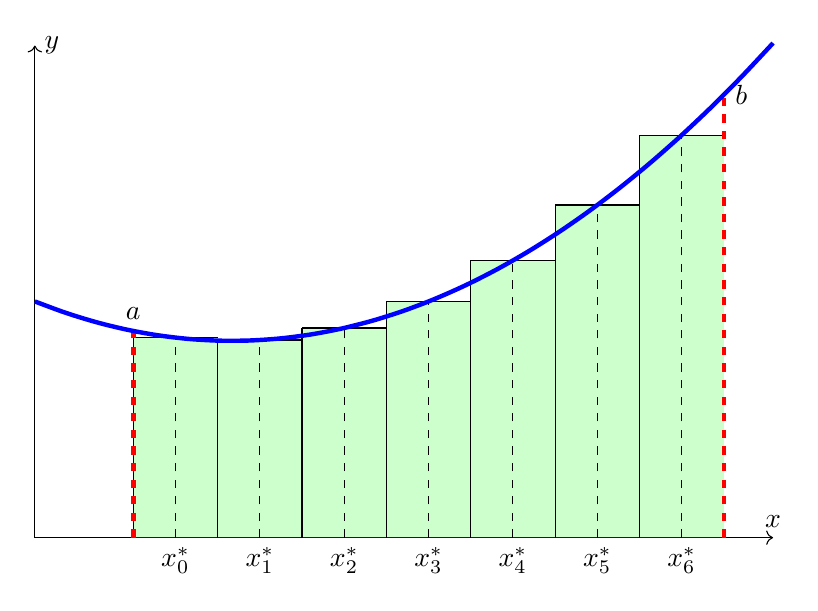
\begin{tikzpicture}[
                scale=1.25,
                declare function={
                    func(\x) = 0.1 * (\x - 2) * (\x - 2) + 2;
                    Width=7.5;
                    Height=5;
                    A = 1;
                    B = 7;
                    N = 7;
                    Delta = {(B-A) / N};
                }
            ]
                \draw[->] (0, 0) -- (0, Height) node[right] {\(y\)};
                \draw[->] (0, 0) -- (Width, 0) node[above] {\(x\)};
        
                \pgfmathtruncatemacro\END{N-1}
                \foreach \x in {0,1,...,\END} {
                    % rectangle
                    \fill [green, opacity=0.2]
                        ({A + Delta * \x}, 0) rectangle ({A + Delta * (\x+1)}, {func(A + Delta * (\x + 0.5))});
                    
                    \draw[-] ({A + Delta * \x}, 0)
                        -- ({A + Delta * \x}, {func(A + Delta * (\x + 0.5))});

                    \draw[-, dashed] ({A + Delta * (\x + 0.5)}, 0)
                        node[below] {\(x_{\x}^*\)}
                        -- ({A + Delta * (\x + 0.5)}, {func(A + Delta * (\x + 0.5))});

                    % line over rectangle
                    \draw[-] ({A + Delta * \x}, {func(A + Delta * (\x + 0.5))})
                        -- ({A + Delta * (\x+1)}, {func(A + Delta * (\x + 0.5))});
                }
        
                \draw[-, dashed, red, ultra thick] (A, 0) -- (A, {func(A)}) node[above, black] {\(a\)};
                \draw[-, dashed, red, ultra thick] (B, 0) -- (B, {func(B)}) node[right, black] {\(b\)};
        
                \draw[domain=0:Width, smooth, variable=\x, blue, ultra thick] plot ({\x}, {func(\x)});
            \end{tikzpicture}
        \end{center}
    \end{wrapfigure}

    We want to find the signed area between \(f(x)\) and the \(x\)-axis between
    the interval \([a;b]\).\\
    One way to do it would be by dividing the area into \(n\) rectangles, each of width
    \[
        \Delta x = \frac{b-a}{n}
    \]
    The height of each triangle is given by \(f(x_k^*)\).
    The area under the curve is approximately
    \[
        A \approx \sum_{k=0}^{n-1}f(x_k^*)\Delta x
    \]
    Notice that the position of \(x_k^*\) within the base of each rectangle controls the type of
    the approximation of the area under the curve.
    By moving \(x_k^*\) within the base we may achieve an approximation by abundance
    or defect.
    The type of approximation does not matter when we let \(n\to \infty\).
    As the amount of rectangles approaches infinity, the approximation approaches
    the exact value of the area.
    \[
        A = \lim_{n\to\infty} \sum_{k=0}^{n}f(x_k^*)\Delta x
    \]
    \wrapfill
\end{snippet}

\begin{snippetproposition}{definite-integral-inversion}{}
    \[
        \integral[a][b][f(x)][x] = -\integral[b][a][f(x)][x]
    \]
\end{snippetproposition}

\begin{snippetcorollary}{fundamental-calculus-theorem-corollary-1}{Non-constant integral limits derivative}
    When the upper or lower limit is not constant,
    \begin{align*}
        \frac{d}{dx} \integral[v(x)][u(x)][f(t)][t]
        &= \frac{d}{dx} \left[ F(u(x)) - F(v(x)) \right] \\
        &= u'(x)f(u(x)) - v'(x)f(v(x))
    \end{align*}
\end{snippetcorollary}

\section{Average Function Value}

\begin{snippetdefinition}{integral-mean-value-definition}{Integral mean value}
    Let \(f\colon [a,b] \to \realnumbers\) integrable on \([a,b]\).
    Then, its \emph{integral mean value} is defined as
    \[
        \frac{1}{b-a} \integral[a][b][f(t)][t]
    \]
\end{snippetdefinition}

\begin{snippettheorem}{integral-mean-value-theorem}{Mean Value Theorem}
    Let \(f\colon [a,b] \to \realnumbers\) integrable on \([a,b]\)
    and let \(M\) be its integral mean value.
    Then,
    \begin{enumerate}
        \item \(\inf_{[a,b]} f \leq M \leq \sup_{[a,b]} f\);
        \item if \(f\) is continuous on \([a,b]\) then \(\exists c\in[a,b]\) such that \(M = f(c)\).
    \end{enumerate}
\end{snippettheorem}

\begin{snippetproof}{integral-mean-value-theorem-proof}{integral-mean-value-theorem}{Mean Value Theorem}
    \begin{enumerate}
        \item Since \(f\) is integrable on \([a,b]\), by definition it is \bounded there,
        \item and for every \(x\in [a,b]\) we have that
        \[
            - \infty < \inf_{[a,b]} f \leq f(x) \leq \sup_{[a,b]} f < +\infty
        \]
        from which, by integrating over \([a,b]\) and using monotonicity, we obtain
        \begin{align*}
            \integral[a][b][\left(\inf_{[a,b]} f\right)][x]
            \leq
            \integral[a][b][f(x)][x]
            \leq
            \integral[a][b][\left(\sup_{[a,b]} f\right)][x]
            \\
            \left(\inf_{[a,b]} f\right)(b-a)
            \leq
            \integral[a][b][f(x)][x]
            \leq
            \left(\sup_{[a,b]} f\right)(b-a)
            \\
            \left(\inf_{[a,b]} f\right)
            \leq
            \frac{1}{b-a}\integral[a][b][f(x)][x]
            \leq
            \left(\sup_{[a,b]} f\right)
        \end{align*}
        \item If \(f\) is continuous on \([a,b]\), then \(\inf f = \min_{[a,b]} f\) and
        \(\sup f = \max_{[a,b]} f\), and from the previous point, we have that
        \[
            \min_{[a,b]} f \leq
            \frac{1}{b-a} \integral[a][b][f(t)][t]
            \leq \max_{[a,b]} f
        \]
        and by the intermediate value theorem, there exists \(c \in [a,b)\) such that
        \[
            f(x) = \frac{1}{b-a} \integral[a][b][f(t)][t]
        \]
    \end{enumerate}
\end{snippetproof}

\begin{snippettheorem}{continuous-function-integral-cancellation-theorem}{}
    Let \(f \colon [a,b] \to \realnumbers\) continuous on \([a,b]\).
    \begin{enumerate}
        \item If \(\forall x \in [a,b]\),
        \[
            \integral[a][x][f(t)][t] = 0
        \]
        then \(f=0\);
        \item if \(f \geq 0\) and \(\int_a^b f(t)\,dt = 0\) then \(f(t)=0\).
    \end{enumerate}
\end{snippettheorem}

\begin{snippetproof}{continuous-function-integral-cancellation-theorem-proof}{continuous-function-integral-cancellation-theorem}{}
    \begin{enumerate}
        \item By the fundamentl theorem of calculus, \(f\) is continuous implies that
        \[
            F(x) = \integral[a][x][f(t)][t]
        \]
        is differentiable and \(F'(x) = f(x)\). By hypothesis, \(\forall x, F(x) = 0\) and thus
        for every \(x\) we have \(0=F'(x) = f(x)\);
        \item let \(f \geq 0\) then \[
            F(x) = \integral[a][x][f(t)][t]
        \]
        is a monotonic increasing \function, thus \(\forall x\in[a,b], F(a) = 0 \leq F(x) \leq F(b)\).
        By hypothesis, \(F(b) = 0\), thus \(F(x) = 0\) for every \(x\). Then, by the previous point,
        we have the thesis.
    \end{enumerate}
\end{snippetproof}

\begin{snippettheorem}{positive-continuous-function-non-zero-integral-theorem}{}
    Let \(f \colon [a,b] \to \realnumbers\) be a \function such that \( f\geq 0\) on \([a,b]\), continuous in \(x_0\)
    and \(f(x_0) > 0\).
    Then,
    \[
        \integral[a][b][f(t)][t] > 0
    \]
\end{snippettheorem}

\section{Area Between Functions}

\begin{snippet}{area-between-functions-illustration}
    \begin{wrapfigure}{l}{7.5cm}
        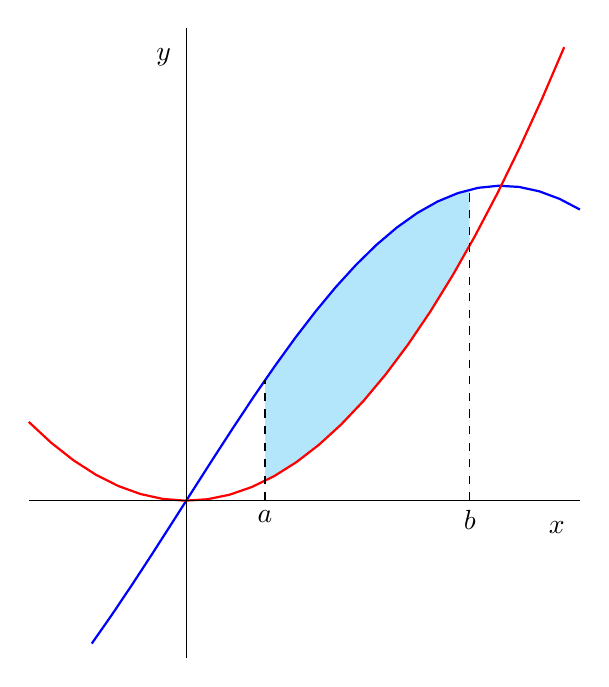
\begin{tikzpicture}[x=4cm, y=4cm, >=Stealth, declare function={
            func1(\x) = sin(3.14*\x/2 r);
            func2(\x) = \x*\x;
            a=0.25;
            b=0.9;
        }]
            % area under func1 
            \fill[cyan!30!white] plot[domain=a:b] (\x,{func1(\x)}) -- plot[domain=b:a] (\x,{0}) -- cycle;
            

            % area under func2
            \fill[white] plot[domain=a:b] (\x,{func2(\x)}) -- plot[domain=b:a] (\x,{0}) -- cycle;
            
            % func1
            \draw[blue, -, thick] plot[domain=-0.3:1.25] (\x,{func1(\x)});
            
            % func2
            \draw[red, -, thick]  plot[domain=-0.5:1.2] (\x,{func2(\x)});

            \draw[-, dashed] (a, 0) node[below] {\(a\)} -- (a, {func1(a)});
            \draw[-, dashed] (b, 0) node[below] {\(b\)} -- (b, {func1(b)});

            \draw[-] (-.5,0) -- (1.25, 0)
                node[below left=4pt and 2pt] {\(x\)};
            \draw[-] (0,-.5) -- (0,1.5)
                node[below left=4pt and 2pt] {\(y\)};
        \end{tikzpicture} 
    \end{wrapfigure}

    Given a \function \(y=f(x)\) and \(y=g(x)\), the area enclosed by the two functions
    in the interval \(I=[a;b]\) is given by
    \[
        A=\integral[a][b][f(x)-g(x)][x]
    \]
    assuming that \(f(x)\geq g(x)\) when \(x\in I\). \\
    Note that \(A\geq 0\). \\
    If \(f(x)<g(x)\) for some \(x\in I\) this formula won't work. However, it is still
    possible to split the integral into multiple integrals at every point where \(f(x) - g(x)\) changes sign.
    To remove the sign contraint we could say
    \[
        A = \integral[a][b][|f(x)-g(x)|][x]
    \]
    \wrapfill
    \vspace{-2.5cm}
    \begin{wrapfigure}{l}{7.5cm}
        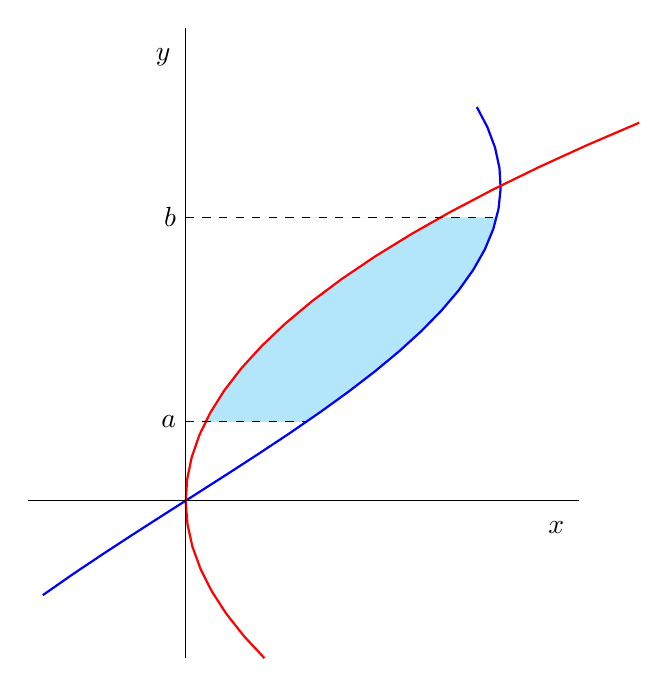
\begin{tikzpicture}[x=4cm, y=4cm, >=Stealth, declare function={
            func1(\x) = sin(3.14*\x/2 r);
            func2(\x) = \x*\x;
            a=0.25;
            b=0.9;
        }]
            % area under func1 
            \fill[cyan!30!white] plot[domain=a:b] ({func1(\x)},\x) -- plot[domain=b:a] ({0}, \x) -- cycle;
            

            % area under func2
            \fill[white] plot[domain=a:b] ({func2(\x)}, \x) -- plot[domain=b:a] ({0}, \x) -- cycle;
            
            % func1
            \draw[blue, -, thick] plot[domain=-0.3:1.25] ({func1(\x)}, \x);
            
            % func2
            \draw[red, -, thick]  plot[domain=-0.5:1.2] ({func2(\x)}, \x);

            \draw[-, dashed] (0, a) node[left] {\(a\)} -- ({func1(a)}, a);
            \draw[-, dashed] (0, b) node[left] {\(b\)} -- ({func1(b)}, b);

            \draw[-] (-.5,0) -- (1.25, 0)
                node[below left=4pt and 2pt] {\(x\)};
            \draw[-] (0,-.5) -- (0,1.5)
                node[below left=4pt and 2pt] {\(y\)};
        \end{tikzpicture} 
    \end{wrapfigure}

    The same thing applies when we have functions in the form \(x=f(y)\) and \(x=g(y)\)
    and we want to find the areas enclosed by the functions when \(y\in [d;c]\)
    \[
        A=\integral[d][c][|f(y)-g(y)|][y]
    \]
    \wrapfill
    \vspace{-2.5cm}
\end{snippet}

\begin{snippetproof}{area-of-circle-theorem-proof}{area-of-circle-theorem}{Area of circle}
    The equation for a circle is \(x^2 + y^2 = r^2\).
    To compute its area, we can consider the function of the upper semicircle
    and compute the area from \(0\) to \(r\). This will prove the area
    of a quarter of the circle. Thus, the full area is given by
    \[
        4\integral[0][r][\sqrt{r^2 - x^2}][x]
    \]
    We substitute \(x = r\sin\theta\), meaning \(dx = r\cos\theta\,d\theta\).
    Note that when \(x=0\), \(\theta = 0\) and when \(x=r\), \(\theta = \picircle / 2\).
    \begin{align*}
        4\integral[0][r][\sqrt{r^2 - x^2}][x]
        &= 4\integral[0][\picircle / 2][\sqrt{r^2 - r^2\sin^2\theta}r\cos\theta][u] \\
        &= 4\integral[0][\picircle / 2][r^2\cos\theta \sqrt{1-\sin^2\theta}][u] \\
        &= 4r^2\integral[0][\picircle / 2][\cos^2\theta][u] \\
        &= 4r^2\integral[0][\picircle / 2][\frac{1 + \cos(2\theta)}{2}][u] = r^2\picircle
    \end{align*}
\end{snippetproof}

\end{document}